%%%%%%%%%%%%%%%%%%%%%%%%%%%%%%%%%%%%%%%%%%%%%%%%%%%%%%%%%%%%%%%%%%%%%%%%%%
%%  CHAPTER 3 -- CARBON POLICIES IN PRODUCTION NETWORKS (JMP)
%%  ~25 minutes. Equations & numbers verbatim from paper/thesis/.
%%%%%%%%%%%%%%%%%%%%%%%%%%%%%%%%%%%%%%%%%%%%%%%%%%%%%%%%%%%%%%%%%%%%%%%%%%

%%%%%%%%%%%%%%%%%%%%% TEMPLATE-STYLE OVERVIEW %%%%%%%%%%%%%%%%%%%%%%%%%%%%
\begin{frame}{Carbon policy in networks: the problem in one slide}

    \begin{tcolorbox}[colback=blue!4,colframe=blue!40!black]
        \textbf{Question:} a carbon price covers \emph{some} firms, not all. What is its
        effect on aggregate emissions, how does that depend on \emph{whom} it covers, and
        is there a firm whose coverage delivers the largest reduction?
    \end{tcolorbox}

    \begin{wideitemize}
        \item[\alertb{Theory:}] GE production network with heterogeneous emission intensities $+$ costly abatement; a carbon price $p_z$ and a $0/1$ coverage vector $\tau$
        \pause
        \item[\alertg{Result:}] $\dfrac{d\log Z}{dp_z}$ decomposes into \alerto{scale} ($\approx 0$), \alertp{technique} (abatement), and \alertb{reallocation} --- the last governed by a \textbf{single covariance} between a firm's policy exposure and its \emph{network-adjusted} emission intensity $\Psi_e$
        \pause
        \item[\alertoch{Data:}] Belgian B2B network $+$ EUTL $\Rightarrow$ under the EU ETS, the cut is \alertr{$\sim$7/8 abatement}, reallocation a modest amplifier
        \pause
        \item[\alertr{Punchline:}] $\sim$94\% of the gain from \emph{whom to cover} comes from firms' \alertr{own} emissions --- a constrained regulator just \alertb{targets the heaviest emitters}
    \end{wideitemize}

\end{frame}

%%%%%%%%%%%%%%%%%%%%% MOTIVATION 1: INCOMPLETE %%%%%%%%%%%%%%%%%%%%%%%%%%
\begin{frame}{Carbon pricing is incomplete by design}

    \begin{columns}
    \begin{column}{0.58\textwidth}
        \begin{figure}
            \centering
            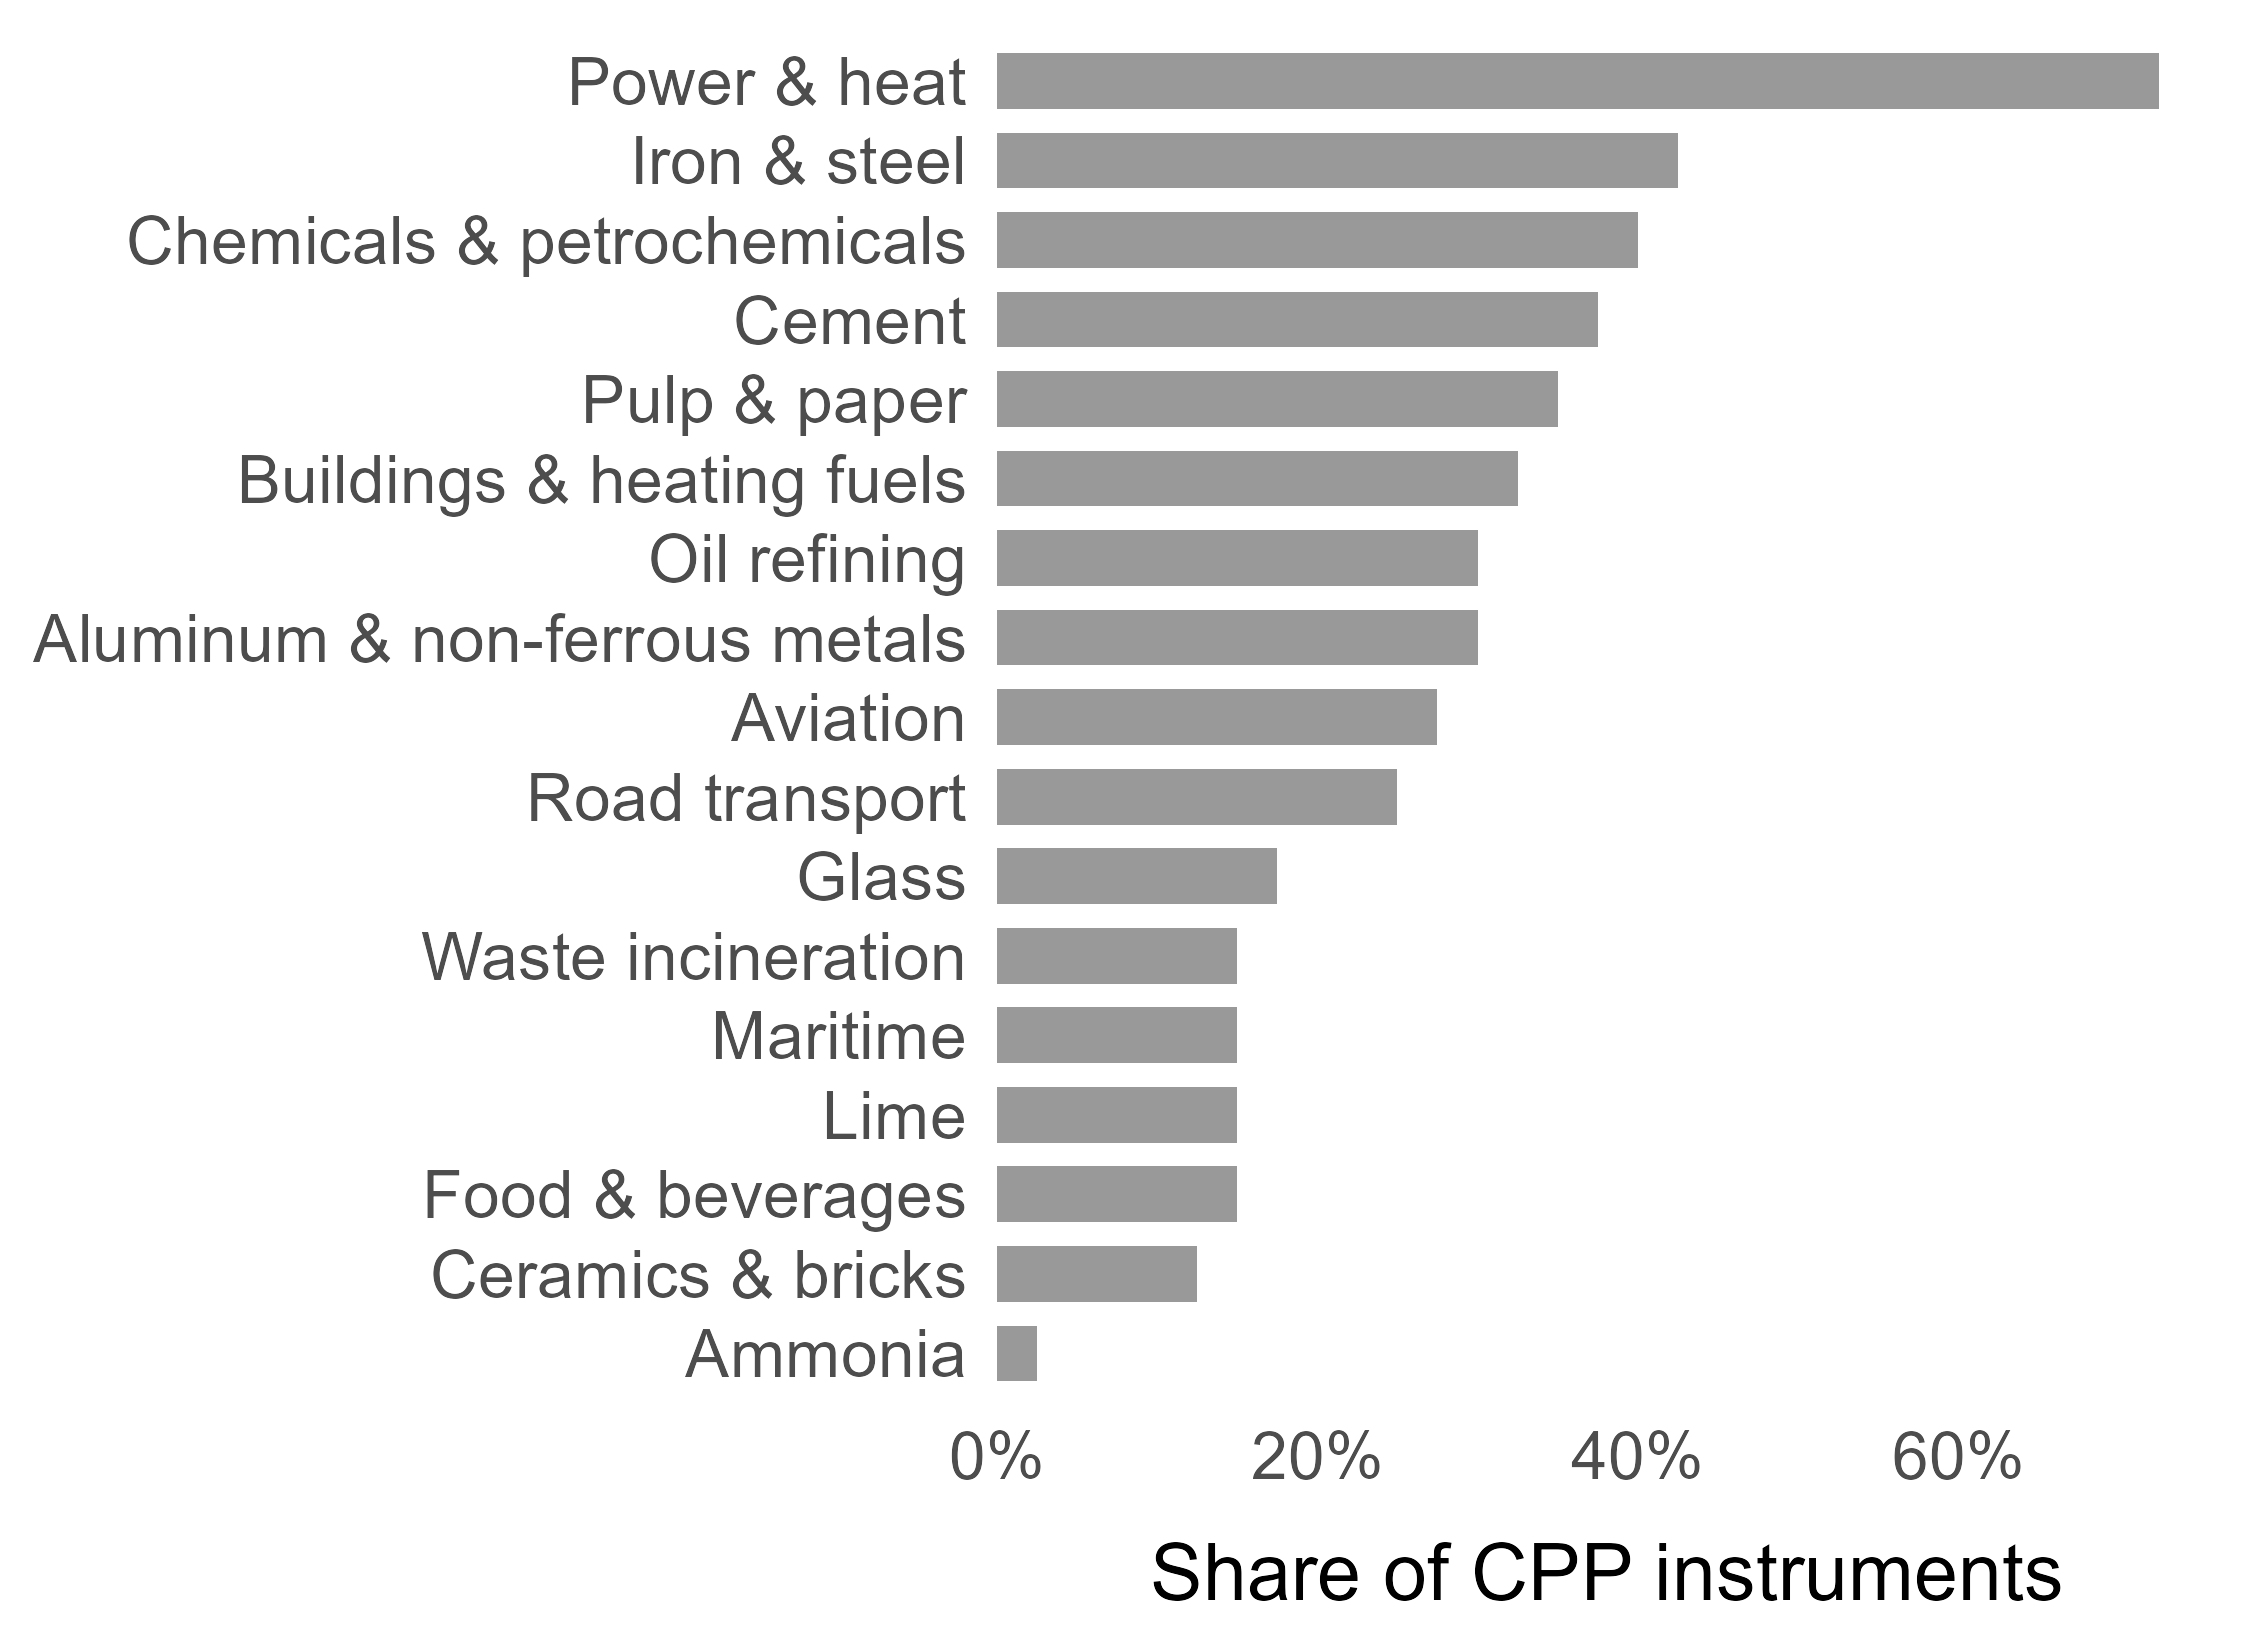
\includegraphics[width=0.99\linewidth]{figures/panel_a_sector_targeting.png}\\[0.2em]
            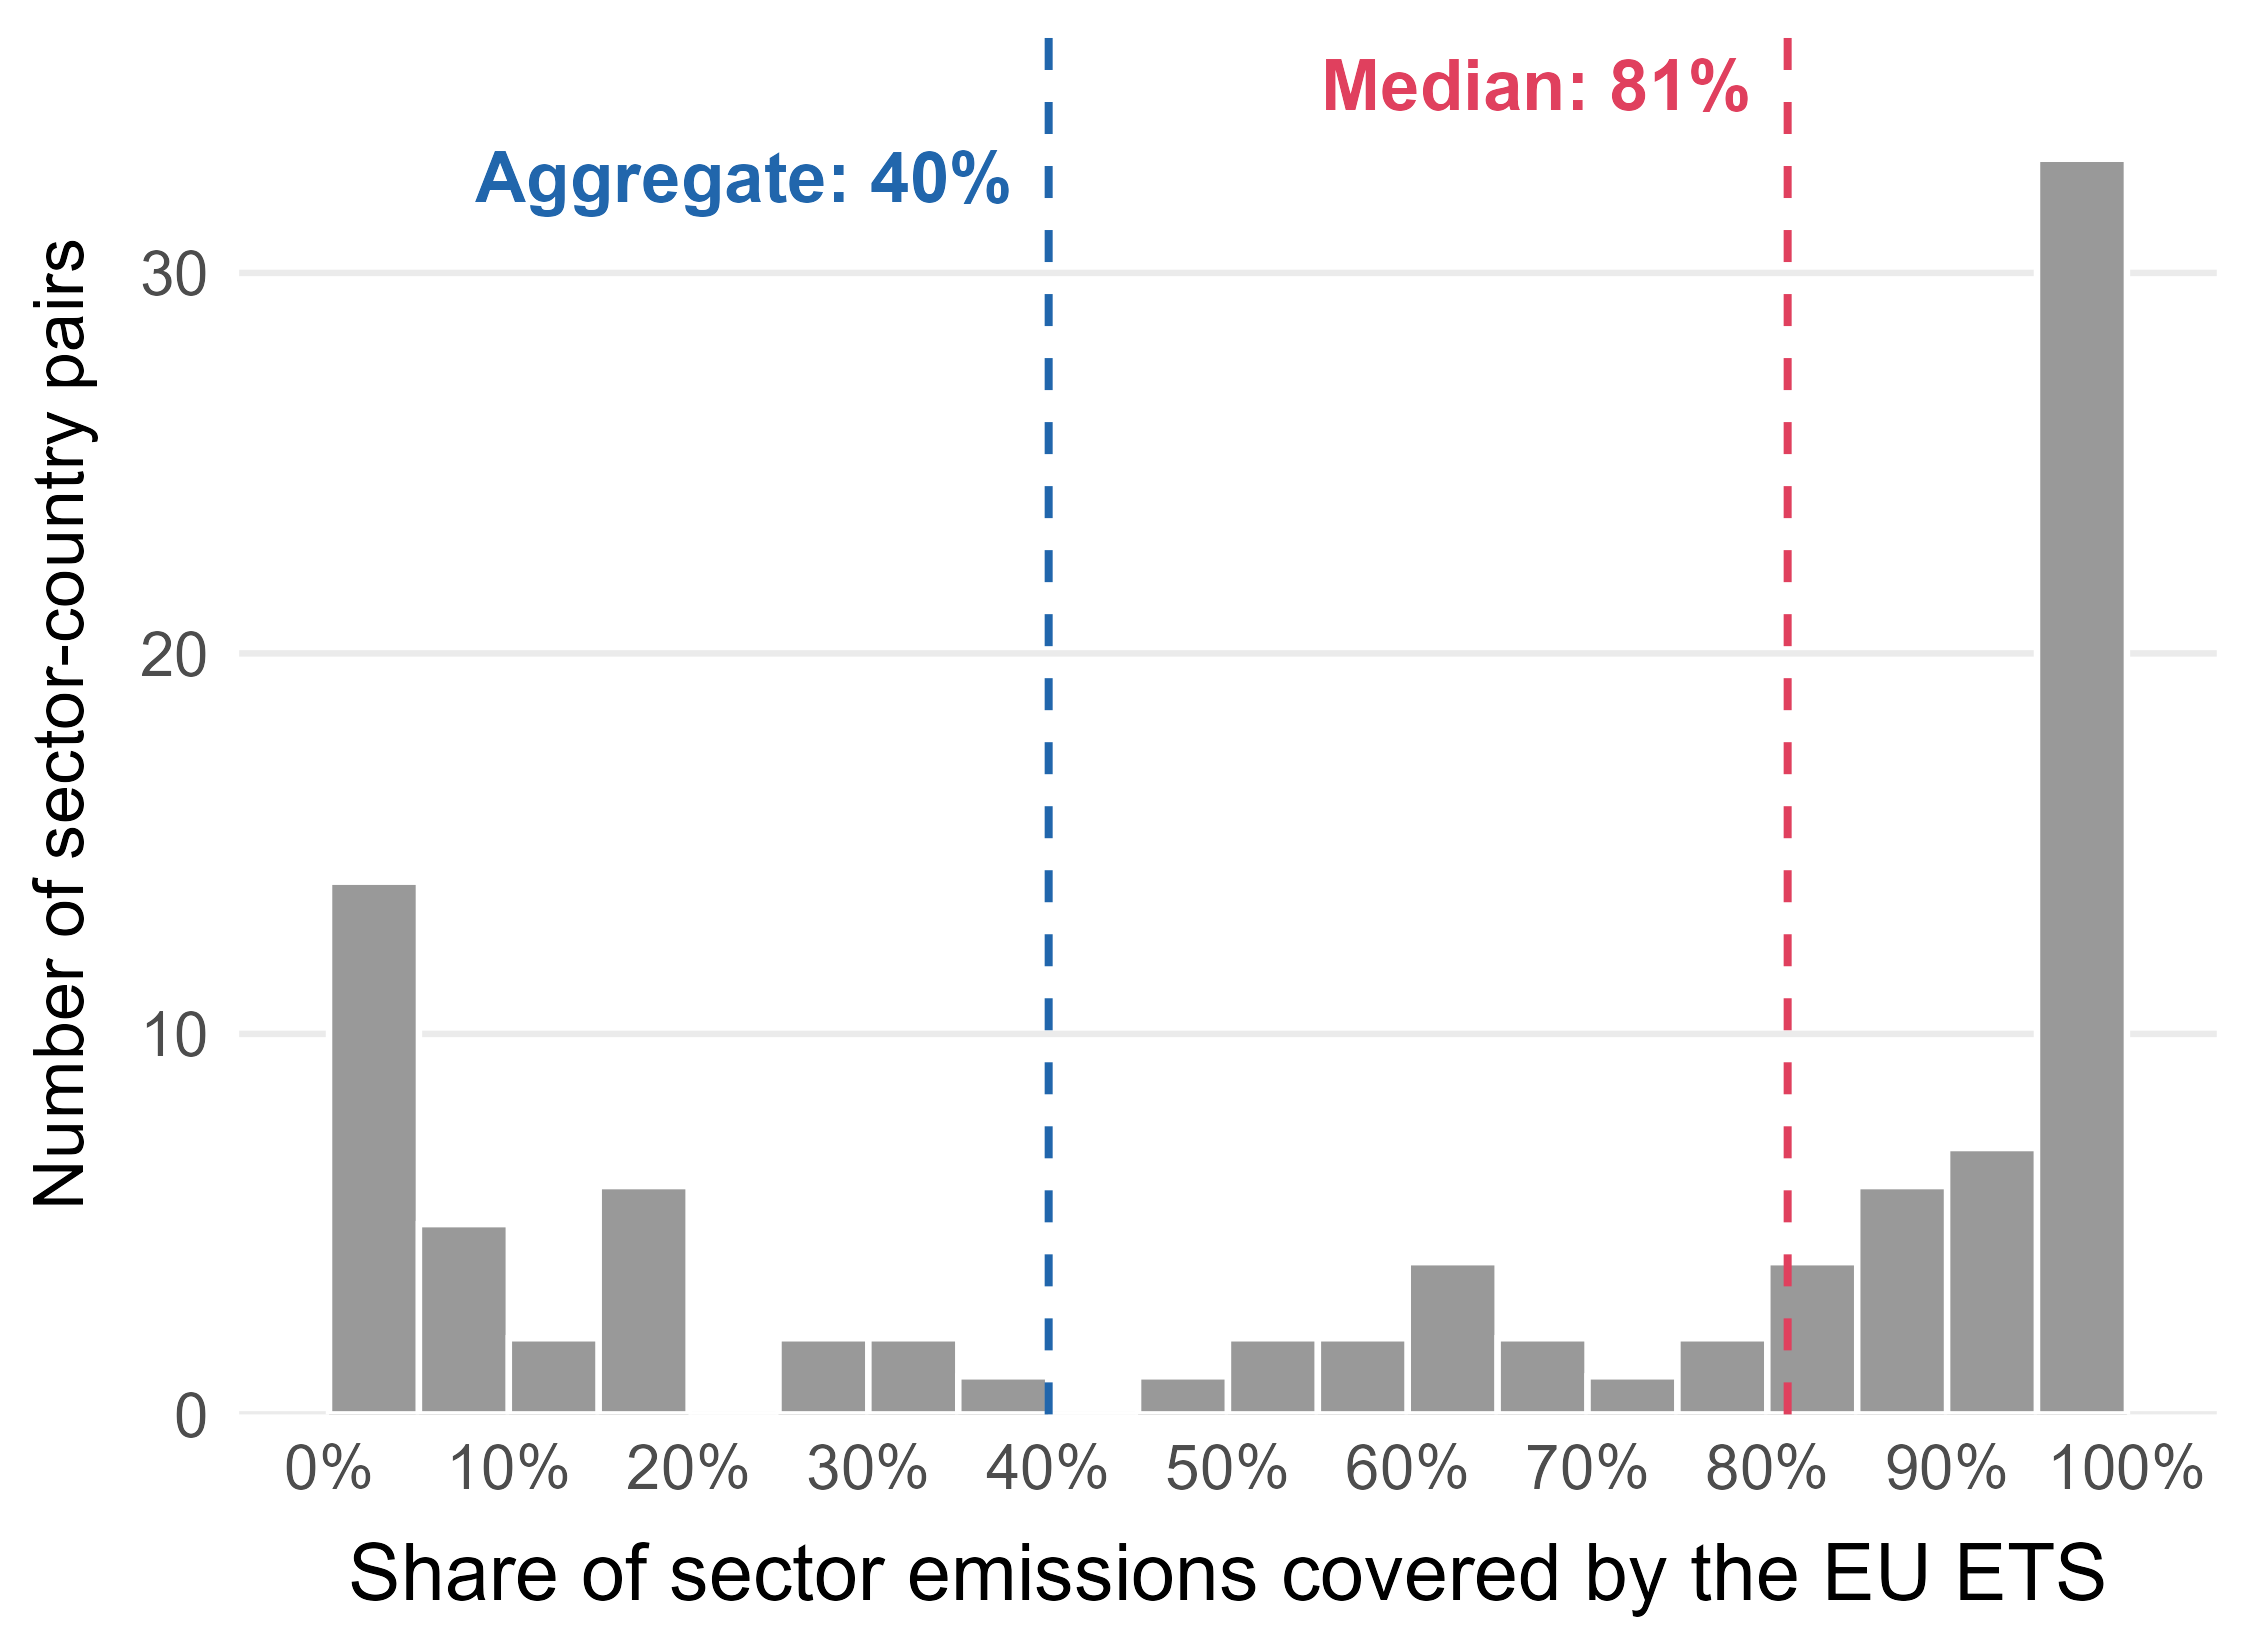
\includegraphics[width=0.99\linewidth]{figures/panel_c_within_sector_coverage.png}
        \end{figure}
    \end{column}
    \begin{column}{0.42\textwidth}
        \begin{wideitemize}
            \item $\sim$75 carbon-pricing instruments in 2024, $\sim$\alertb{a quarter} of global emissions
            \item Coverage is \alerto{partial and uneven} across \emph{and} within sectors
            \item EU ETS: median targeted sector $\sim$80\% priced, but only $\sim$\alertr{40\%} of emissions priced in aggregate
            \item[] \alertg{$\Rightarrow$} incompleteness is the rule, not the exception
        \end{wideitemize}
    \end{column}
    \end{columns}

\end{frame}

%%%%%%%%%%%%%%%%%%%%% MOTIVATION 2: WHY NETWORK %%%%%%%%%%%%%%%%%%%%%%%%%
\begin{frame}{Why the production network matters}

    Three questions: \alertb{(1)} effect of a scheme on aggregate emissions?
    \alertb{(2)} how does it depend on \emph{who} is covered?
    \alertb{(3)} is there a firm whose coverage reduces emissions most?

    \vspace{0.3cm}
    \begin{wideitemize}
        \item A firm's emissions are partly \alertp{its own}, partly \alerto{embodied in the inputs it buys}
        \begin{wideitemize}
            \item[\alertp{1.}] \alertp{Who is exposed} to a carbon price is a network object (taxing one firm reaches beyond it)
            \item[\alerto{2.}] The \alerto{aggregate effect} depends on where dirty firms sit in the network
        \end{wideitemize}
        \item[] The object that matters: \alertg{network-adjusted emission intensity}
        $$ \Psi_e := \Psi\,\overline{\mathcal{E}}, \qquad \Psi = (I-\Omega)^{-1} \quad \text{(direct $+$ upstream-embodied; scope 1$+$2$+$3)} $$
    \end{wideitemize}

\end{frame}

%%%%%%%%%%%%%%%%%%%%% ENVIRONMENT / SETUP %%%%%%%%%%%%%%%%%%%%%%%%%%%%%%%
\begin{frame}{Environment}

    \begin{wideitemize}
        \item Closed economy: household, government, $N$ producers (CRS, marginal-cost pricing $p_i=mc_i$)

        \item \alertb{Policy}: carbon price $p_z$ and coverage vector $\tau=\{\tau_i\}$, $\tau_i\in\{0,1\}$

        \item Producer $i$: Cobb--Douglas in labor and a \alertp{nested-CES} input bundle
        \begin{wideitemize}
            \item[-] across sectors $\sigma_B$ (weak substitution), within sector $\sigma_W$ (stronger)
        \end{wideitemize}

        \item \alertg{Network objects}: input--output matrix $\Omega$, Domar weights $\lambda_i$, Leontief inverse $\Psi=(I-\Omega)^{-1}$

        \item Emissions a by-product of production: $z_i = e_i f_i$, intensity $\overline{e}_i$ in the no-policy economy
    \end{wideitemize}

\end{frame}

%%%%%%%%%%%%%%%%%%%%% ABATEMENT / TECHNIQUE %%%%%%%%%%%%%%%%%%%%%%%%%%%%%
\begin{frame}{Firms abate: the technique channel}

    \begin{wideitemize}
        \item A covered firm pays $p_z$ per unit of emissions $\Rightarrow$ it \alertb{abates}: chooses effort $\kappa_i$
        $$ e_i = (1-\kappa_i)^{\alpha_i}\,\overline{e}_i $$
        {\small $\alpha_i$ governs \alerto{how hard firm $i$ is to abate} (disciplined from abatement-elasticity estimates)}

        \item To first order, the \alertp{technique response}:
        $$ \frac{d \log e_i}{d p_z}\bigg|_{p_z=0} = -\,\tau_i\,\alpha_i^2\,\overline{e}_i \;<\;0 $$

        \item \alertg{Key separability}: abatement lowers intensity but leaves the firm's \emph{input mix} (hence pass-through) unchanged to first order
    \end{wideitemize}

\end{frame}

%%%%%%%%%%%%%%%%%%%%% PRICE PROPAGATION %%%%%%%%%%%%%%%%%%%%%%%%%%%%%%%%%
\begin{frame}{The carbon price propagates through prices}

    \begin{wideitemize}
        \item Each firm passes its carbon cost into its price; buyers inherit it through their inputs:
        $$ \frac{d \log p_i}{d p_z} = \sum_{j\in\N}\Omega_{ij}\,\frac{d \log p_j}{d p_z} \;+\; \Omega_{iL}\,\frac{d \log w}{d p_z} \;+\; \tau_i\,\overline{e}_i $$

        \item In matrix form (the \alertb{exposure} of every price to the policy):
        $$ \frac{d \log \mathbf{p}}{d p_z} = \Psi\,(\tau \circ \overline{\mathcal{E}}) \;+\; \Psi_{(:,L)}\frac{d \log \lambda_L}{d p_z} $$

        \item[] \alertg{$\Rightarrow$} a firm's exposure is its \emph{covered, network-weighted} upstream emission content --- itself a $\Psi$ object
    \end{wideitemize}

\end{frame}

%%%%%%%%%%%%%%%%%%%%% THREE-CHANNEL DECOMPOSITION %%%%%%%%%%%%%%%%%%%%%%%
\begin{frame}{Decomposition: scale, technique, reallocation}

    \begin{wideitemize}
        \item Aggregate emissions move through three channels (Grossman--Krueger accounting, mapped to primitives):
        $$ \frac{d \log Z}{d p_z}\bigg|_{0}
            = \underbrace{\sum_{i\in\N}\frac{z_i}{Z}\frac{d\log e_i}{d p_z}}_{\text{\alertp{technique (abatement)}}}
            \;+\; \underbrace{\sum_{i\in\N}\frac{z_i}{Z}\Big[\tfrac{d\log\lambda_i}{d p_z}-\tfrac{d\log p_i}{d p_z}\Big]}_{\text{\alertb{reallocation}}} $$

        \item \alerto{Scale} $\approx 0$: by Hulten, $\dfrac{d\log Y}{d p_z}\Big|_{0}=0$ --- to first order the policy is a pure pollution-cutting device, not an output story

        \item \alertp{Technique} is set by \emph{covered} firms; \alertb{reallocation} is where the network enters
    \end{wideitemize}

\end{frame}

%%%%%%%%%%%%%%%%%%%%% THE THEOREM %%%%%%%%%%%%%%%%%%%%%%%%%%%%%%%%%%%%%%%%
\begin{frame}{Main result: a sufficient-statistic decomposition}

    \begin{tcolorbox}[colback=blue!4,colframe=blue!45!black]
    $$ \frac{d \log Z}{d p_z}\bigg|_{p_z=0}
        = \underbrace{-\sum_{i \in \N} \frac{\tau_i z_i}{Z}\,\alpha_i^2\,\overline{e}_i}_{\text{\alertp{technique} $<0$, covered firms}}
        \;\underbrace{-\,\sigma \sum_{i \in \N \cup \{C\}} \frac{x_i}{Z}\,\mathbb{C}_{\Omega_{(i,:)}}\!\left(\frac{d \log \mathbf{p}}{d p_z},\,\Psi_e\right)}_{\text{\alertb{reallocation}: one covariance}} $$
    \end{tcolorbox}

    \begin{wideitemize}
        \item Across each buyer's inputs: covariance between \alertb{exposure} ($\tfrac{d\log\mathbf p}{dp_z}$) and \alertg{network-adjusted intensity} $\Psi_e$
        \item Its \alertr{sign} decides whether the network \alertg{amplifies} ($\mathbb{C}>0$) or \alerto{leaks} ($\mathbb{C}<0$)
        \item $(1-\sigma)$ governs the \alertp{magnitude}, not the sign
        \item[] \alertr{Complete coverage} ($\tau=\mathbf 1$): covariance $\to$ \alertg{variance} $\Rightarrow$ reallocation \emph{always} amplifies
    \end{wideitemize}

\end{frame}

%%%%%%%%%%%%%%%%%%%%% EMISSION CENTRALITY %%%%%%%%%%%%%%%%%%%%%%%%%%%%%%%
\begin{frame}{Whom to cover? Emission centrality}

    \begin{wideitemize}
        \item The decomposition is \alertb{additively separable} across covered firms $\Rightarrow$ define the marginal value of covering firm $j$ alone:
        $$ \text{Centrality}_j \;=\; -\frac{z_j}{Z}\,\alpha_j^2\,\overline{e}_j
            \;-\; \sigma \sum_{i \in \N \cup \{C\}} \frac{x_i}{Z}\,\mathbb{C}_{\Omega_{(i,:)}}\!\Big(\Psi_{(:,j)}\,\overline{e}_j,\ \Psi_e\Big) $$

        \item \alertp{Own-abatement} term ($z_j$, $\overline e_j$) $+$ a \alertb{network-position} term
        \item This is the object counterfactuals \alertg{rank firms on} --- and it makes the network's value an \emph{empirical} question
    \end{wideitemize}

\end{frame}

%%%%%%%%%%%%%%%%%%%%% FACTS THAT DISCIPLINE %%%%%%%%%%%%%%%%%%%%%%%%%%%%%%
\begin{frame}{Taking it to Belgian data: facts that discipline the model}

    \begin{columns}
    \begin{column}{0.5\textwidth}
        \begin{figure}
            \centering
            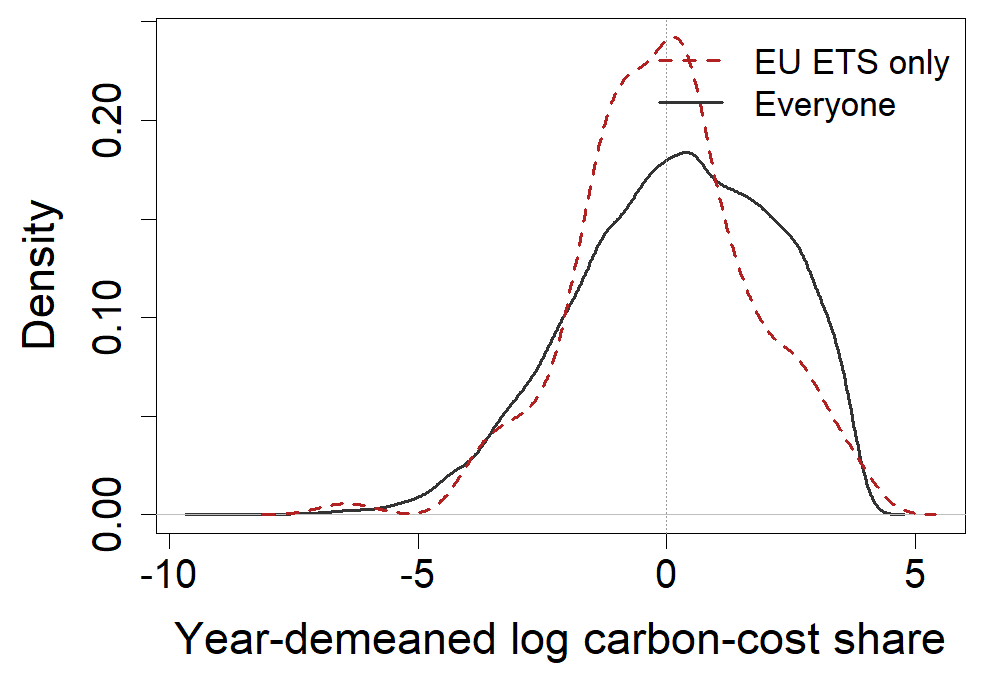
\includegraphics[width=0.92\linewidth]{figures/emission_cost_share_firm_p80.png}
        \end{figure}
    \end{column}
    \begin{column}{0.5\textwidth}
        \begin{wideitemize}
            \item At $p_z=80$: median emitter's carbon cost $\approx$ \alertb{2.5\%} of total cost; $\sim$1 in 6 exceed 20\%
            \item Wide \alerto{dispersion} in direct intensity: within (4d, year) $p_{90}/p_{10}\!\approx\!5.7$; $\to\!\sim$30-fold with the imputed tail
            \item Direct $\leftrightarrow$ upstream link is \alertr{weak} (Spearman $0.24$--$0.33$)
            \item For \alertb{1 in 3} ETS firm-years, \emph{upstream} emissions exceed own direct
        \end{wideitemize}
    \end{column}
    \end{columns}

    \vspace{0.1cm}
    {\footnotesize Thin within-sector supplier base ($\sim$1.5 suppliers/sector) vs.\ broad across-sector base ($\sim$25 sectors sourced) $\Rightarrow$ $\sigma_W>\sigma_B$.}

\end{frame}

%%%%%%%%%%%%%%%%%%%%% CALIBRATION %%%%%%%%%%%%%%%%%%%%%%%%%%%%%%%%%%%%%%%%
\begin{frame}{Calibration}

    \begin{wideitemize}
        \item 2019 Belgian firm-level network ($\Omega$, $\lambda$) from B2B $+$ imports $+$ balance sheets; intensities $\overline{\mathcal E}$ from EUTL ($+$ imputation for the non-ETS tail)

        \item Realized \alertb{EU ETS} coverage $\tau$; carbon price $p_z = $ \alerto{80 EUR/t} (2022 EUA)

        \item Benchmark elasticities:
        $$ \sigma_B = 0.1, \qquad \sigma_W = 2.5, \qquad \rho = 0.7, \qquad \alpha = 2 $$
        {\small ($\rho$: incomplete pass-through, a Katz--Bonacich Leontief $\Psi_\rho$; $\alpha$ from abatement-elasticity estimates. Robustness over grids on each.)}
    \end{wideitemize}

\end{frame}

%%%%%%%%%%%%%%%%%%%%% RESULT 1: EU ETS DECOMP %%%%%%%%%%%%%%%%%%%%%%%%%%%
\begin{frame}{Result 1 --- the EU ETS effect is mostly abatement}

    \begin{center}
    \begin{tabular}{lcc}
    \toprule
    Channel & $\Delta\log Z$ & share \\
    \midrule
    \textbf{Total}            & \alertb{$-0.421$} & \\
    \quad Scale               & $-0.000$ & $\approx 0$ \\
    \quad \alertp{Technique}  & \alertp{$-0.371$} & $\approx 88\%$ (\,$\sim$7/8\,) \\
    \quad \alertb{Composition}& \alertb{$-0.049$} & $\approx 12\%$ \\
    \bottomrule
    \end{tabular}
    \end{center}

    \begin{wideitemize}
        \item Composition is \alertg{negative} $\Rightarrow$ the Belgian network \alertg{amplifies} abatement (covariance positive: covered firms are positioned in cleaner-leaning supply chains)
        \item But \alerto{uneven}: taxing a firm lowers emissions at \alertb{$\sim$4 in 5} firms, raises them at the rest --- the raisers offset \alertr{$\sim$1/5} of the reductions
        \item For \alertr{$\sim$1 in 25} firms, coverage \emph{backfires}: demand shifts to dirtier uncovered rivals
    \end{wideitemize}

\end{frame}

%%%%%%%%%%%%%%%%%%%%% RESULT 2: WHICH VS HOW MANY %%%%%%%%%%%%%%%%%%%%%%%
\begin{frame}{Result 2 --- \emph{which} firms beats \emph{how many}}

    \begin{columns}
    \begin{column}{0.44\textwidth}
        \begin{figure}
            \centering
            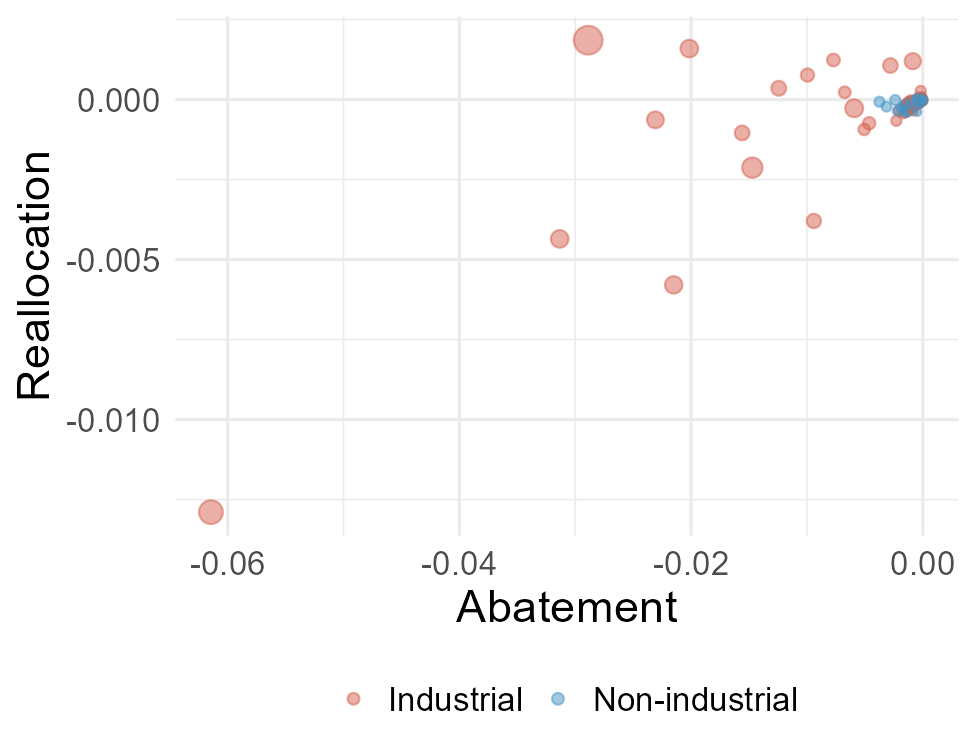
\includegraphics[width=0.86\linewidth]{figures/centrality_plane.png}
        \end{figure}
        {\scriptsize Technique vs.\ composition centrality (corr.\ $0.74$).}
    \end{column}
    \begin{column}{0.56\textwidth}
        \begin{wideitemize}
            \item Re-selecting the \emph{same number} of firms toward central ones: \alertg{$+31.7\%$} vs.\ ETS
            \item Expanding to \emph{all} of industry: only \alerto{$+5.3\%$}
            \item[] \alertb{$\Rightarrow$ \emph{which} $\approx$ 6$\times$ \emph{how many}}
        \end{wideitemize}
    \end{column}
    \end{columns}

    \begin{tcolorbox}[colback=blue!4,colframe=blue!45!black,boxsep=2pt,top=3pt,bottom=3pt]
    \footnotesize \textbf{But:} holding firm count fixed, ranking on \alertr{direct emissions $z_i$ alone}
    recovers \alertr{$\sim$94\%} of the centrality gain --- the network's extra value sits at the
    \emph{backfiring} margin, not in everyday selection.
    \end{tcolorbox}

\end{frame}

%%%%%%%%%%%%%%%%%%%%% CONCLUSION %%%%%%%%%%%%%%%%%%%%%%%%%%%%%%%%%%%%%%%%%
\begin{frame}{Chapter 3 --- takeaways}

    \begin{wideitemize}
        \item A \alertb{transparent decomposition} of targeted carbon pricing in a network: scale ($\approx 0$), technique, and reallocation --- the last a \alertg{single covariance} of exposure with network-adjusted intensity $\Psi_e$

        \item Empirically (Belgium, EU ETS): the cut is \alertp{$\sim$7/8 abatement}; the network \alertg{amplifies} modestly

        \item The network is indispensable for \alertb{diagnosis} --- measuring the effect and flagging the $\sim$1-in-25 firms that backfire --- but for \alerto{selection} a constrained regulator simply \alertr{targets the heaviest emitters}

        \item[] \alertp{Next}: open economy (cross-border leakage --- Chapter~2), and the jointly-optimal covered set
    \end{wideitemize}

\end{frame}
